%%%%%%%%%%%%%%%%%%%%%%%%%%%%%%%%%%%%%%%%%%%%%%%%%%%%%%%
% A template for Wiley article submissions.
% Developed by Overleaf. 
%
% Please note that whilst this template provides a 
% preview of the typeset manuscript for submission, it 
% will not necessarily be the final publication layout.
%
% Usage notes:
% The "blind" option will make anonymous all author, affiliation, correspondence and funding information.
% Use "num-refs" option for numerical citation and references style.
% Use "alpha-refs" option for author-year citation and references style.

\documentclass[alpha-refs]{wiley-article}
% \documentclass[blind,num-refs]{wiley-article}

% Add additional packages here if required
\usepackage{siunitx}
\usepackage{comment}
\usepackage{xcolor}
\usepackage{amsmath}
\usepackage{setspace}
\doublespacing
\usepackage{lineno}
\linenumbers 

% Update article type if known
\papertype{Original Article}
% Include section in journal if known, otherwise delete
\paperfield{Journal Section}

\title{Forecast Verification for Land-Sea Breeze and Boundary Layer Mixing Processes}

% Include full author names and degrees, when required by the journal.
% Use the \authfn to add symbols for additional footnotes and present addresses, if any. Usually start with 1 for notes about author contributions; then continuing with 2 etc if any author has a different present address.
\author[1]{Ewan Short}
\author[2]{Ben Price}
\author[3]{Derryn Griffiths}
\author[3]{Alexei Hider}
%\author[2\authfn{2}]{Author Three PhD}
%\author[2]{Author B.~Four}

%\contrib[\authfn{1}]{Equally contributing authors.}

% Include full affiliation details for all authors
\affil[1]{ARC Centre of Excellence for Climate Extremes, School of Earth Sciences, University of Melbourne, Parkville, VIC, 3010, Australia}
\affil[2]{Bureau of Meteorology, Casuarina, NT, 0810, Australia}
\affil[3]{Bureau of Meteorology, Melbourne, VIC, 3208, Australia}

\corraddress{Ewan Short, ARC Centre of Excellence for Climate Extremes, School of Earth Sciences, University of Melbourne, Parkville, VIC, 3010, Australia}
\corremail{ewan.short@unimelb.edu.au}

%\presentadd[\authfn{2}]{Department, Institution, City, State or Province, Postal Code, Country}

\fundinginfo{ARC Centre of Excellence for Climate System Science}

% Include the name of the author that should appear in the running header
\runningauthor{Ewan Short et al.}

\begin{document}

\maketitle

\begin{abstract}
This study presents a methodology for comparing the performance of Australian Bureau of Meteorology forecasts of the land-sea breeze with unedited model guidance products, such as those of the European Center for Medium-Range Weather Forecasting (ECMWF) and the Australian Community Climate and Earth System Simulation (ACCESS). The methodology is applied to the 8 Australian capital city airports. The results indicate that at some airports, human intervention to model guidance products adds value to land-sea breeze forecasts, whereas at other airports it does not. 

% Please include a maximum of seven keywords
\keywords{land-sea breeze, forecast verification, Australia, ACCESS, ECMWF}
\end{abstract}

\section{Introduction}\label{introduction}
Modern weather forecasts are produced by models in conjunction with human forecasters. For instance, a forecaster working for the Australian Bureau constructs a seven day forecast by first loading model data into the Graphical Forecast Editor (GFE) software package, then manually editing this model data as they see fit. Forecasters can choose which model to base their forecast on, and refer to this as a choice of \textit{model guidance}. Edits are typically made to account for processes that are underesolved at synoptic scale model resolutions, or to address known biases of the models being used. 

It is therefore important to assess not only the overall accuracy of weather forecasts, but also the contribution human forecaster edits make to this accuracy. If effective, but routine, editing procedures can be identified they can be automated, freeing forecasters up to focus on other tasks. One common edit involves changing the surface wind fields near coastlines to try to represent sea-breezes more realistically. Forecasters invest time in making sea-breeze edits because accurate predictions of near-surface winds are highly valued by a number of users, such as the aviation and energy \citep{smith09} industries. Accurate sea-breeze forecasts are also valuable to environmental monitoring authorities, as these winds provide ventilation to coastal urban areas.

Assessing the accuracy of a weather forecast is a task far more nuanced than it might first appear. For instance, attempting to assess the accuracy of a precipitation forecast by comparing the rainfall amounts measured at an individual weather station to the closest grid point of a model prediction will often give poor results. Although the synoptic drivers of convection are usually well predicted, excatly where convective cells form, and where the most rain falls, is highly unpredictable. As such, it is often appropriate to use ``fuzzy" verification metrics which measure the agreement between prediction and observation in a more indirect way. For instance, one approach known as ``upscaling" is to first average forecast and observational data over a given spatial domain before calculating verification scores. \citet{ebert08} provided a review of current ``fuzzy verification" methodologies, and a framework for how they can be used to determine the spatial scales at which a given forecast has predictive skill.      

Relatively few forecast verification studies have focused on near-surface winds, and the ones that have generally only considered wind speeds. \citet{pinson12} performed a verification study of the ECMWF 10 m wind speeds across western Europe over December, January, February 2008/09. First, they interpolated ECMWF model data onto the locations of weather stations across Europe, then they compared the interpolated model data at these stations with the station observations themselves. They found that the worst performing regions were coastal and mountainous areas, and attributed this poor performance to the small scale processes, e.g. sea and mountain breezes, that are underesolved at ECMWF's coarse 50km spatial resolution. They noted that future work could better identify the effect of diurnal cycles on verification statistics by considering forecasts at different times of day. 

\citet{lynch14} also performed a verification study of ECMWF 10 m wind speed data, with the goal of assessing skill at lead times of between 14 to 20 days. They compared ECMWF 32-day forecast model wind speeds with gridded ERA-Interim wind speeds between 2008-12, with both datasets analysed at a six hour temporal resolution. Before conducting the comparison, the wind speed data were transformed into wind-speed ``anomaly" data by first calculating the mean wind speed at 0000, 0600, 1200 and 1800 UTC for each calendar day from the entire ERA-Interim record, and from a 20 year ECMWF 32-day model hindcast, then subtracting these means from the ERA-Interim and ECMWF 32-day model data respectively. Wind speed anomaly data was used so that stable seasonal and diurnal cycles did not contribute to verification scores. At the 14-20 day timescale around western Europe, the greatest skill was found in the boreal winter (austral summer) months of December, January and February.  

\citet{pinson12} and \citet{lynch14} restricted their verification studies to wind speeds, but wind directions are also crucial to diagnosing whether land sea breezes - and the diurnal wind cycle more generally - are being forecast correctly. Furthermore, no previous published work has proposed a verification methodology to assess the accuracy of the diurnal wind cycle in forecasts, or of the contributions made to this accuracy by human forecaster edits of model output. Finally, no previously published work has considered the performance of ACCESS near surface winds, which together with ECMWF, are the model guidance products most widely used by Australian forecasters. Thus, the present study has two goals. First, to describe a methodology for comparing human edited forecasts of the land-sea breeze to unedited model guidance forecasts, in order to assess where and when human edits are producing an increase in accuracy. Second, to apply this methodology across Australia. The remainder of this paper is organised as follows. Section \ref{methods} describes the methodology in detail, section \ref{results} provides results, and sections \ref{discussion} and \ref{conclusion} provide a discussion and a conclusion, respectively.     

\section{Data and Methods} \label{Sec:Methods}
This study compares both edited and non-edited Australian Bureau of Meteorology forecast data with automatic weather station (AWS) data across Australia. The comparison is performed by first isolating the diurnal signals of each dataset, then comparing these signals on an hour-by-hour basis. \textcolor{red}{If the diurnal cycle cannot be resolved correctly using wind perturbations, it cannot be resolved correctly in the overall wind fields, which are subject to additional synoptic scale errors between the models and observations.}

\subsection{Data} 
Four datasets are considered in this study; they are the Australian Bureau of Meteorology's Official wind forecast data, model data from the European Center for Medium Range Weather Forecasting (ECMWF), model data from the Australian Community Climate and Earth System Simulator (ACCESS), and observational data from automatic weather stations. The Official, ECMWF and ACCESS data are at a \textcolor{red}{?, ?} degree spatial resolution respectively. \textcolor{red}{What are the resolutions of these datasets as they're used in Jive? Does the ACCESS model data in Jive} Official, ACCESS and AWS data exists at each UTC hour. ECMWF data exists at a three hour resolution. To be consistent with the other data sets, ECMWF is therefore linearly interpolated to an hourly resolution: this is also what happens in practice when forecasters load ECMWF wind data into the GFE. Two time periods are considered, the austral summer months (December, January, February) of 2017/18, and the austral winter months (June, July, August) of 2018. 

\begin{figure}
\centering
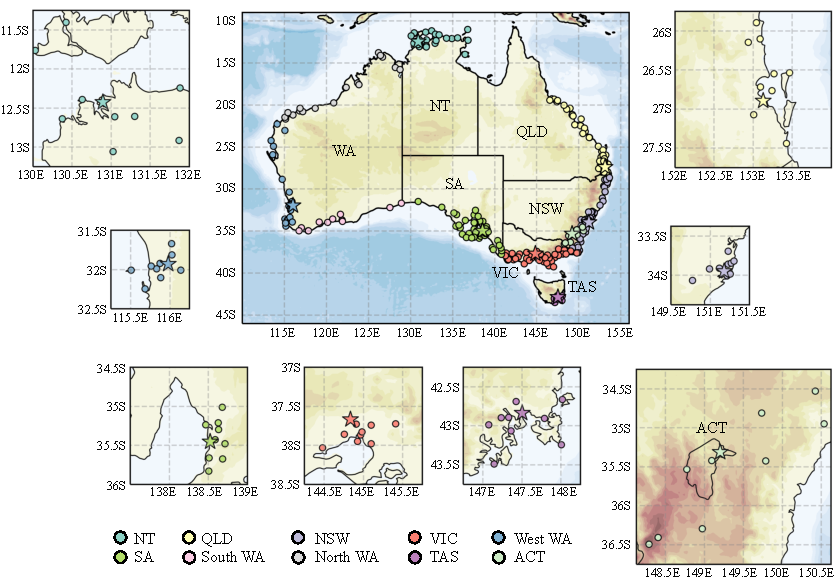
\includegraphics{map.pdf}
\caption{Locations of the automatic weather stations used in this study. Stars indicate capital city airport stations. Height and depth shading intervals every 200 and 1000 m, respectively.}
\label{Fig:map}
\end{figure}

Only station data from the seven Australian capital city airport automatic weather stations are considered; Official, ECMWF and ACCESS  data is \textcolor{red}{(linearly?)} interpolated to the coordinates of the airport weather stations. Capital city airports have been chosen as the focus of this study for a number of reasons. Automatic weather stations located at airports tend to provide the most accurate wind data, and wind forecasts at airports are important to the aviation industry. Moreover, the capital city airports are all reasonably close to coastlines, resulting in a clear diurnal signal. Finally, these airports are also all close to their respective capital cities, which are high priority regions for accurate forecasting. The datasets are hosted on the Bureau's Jive database, but are not currently generally available, although the long term plan is for this to change. \textcolor{red}{Can I extract and host the data I need myself? Can I obtain copies of the relevant Jive Functions so that I can post complete code online?}

As described above, the Australian Bureau of Meteorology's official wind forecast is constructed out of model data, which is then edited by human forecasters using the Graphical Forecast Editor (GFE) software package. Australian forecasters typically construct wind forecasts out of model data either from the European Center for Medium Range Weather Forecasting (ECMWF), or the Australian Community Climate and Earth System Simulator (ACCESS). Testing whether the official forecast data conforms more closely to the AWS observations than ECMWF or ACCESS therefore provides a way to assess the extra accuracy gained by forecaster edits.

\subsection{Assessing Diurnal Cycles}
Although close to coastlines the land-sea breeze is generally the dominant diurnal wind process, the overall diurnal signal may also include mountain-valley breezes, boundary layer mixing processes, atmospheric tides, and urban heat island circulations. Forecasters typically edit model output to account for \emph{both} unresolved sea-breezes \emph{and} unresolved boundary layer mixing; attempting to focus solely on sea-breezes without examining the entire diurnal cycle therefore risks erroneous conclusions, with the effects of one category of edit mistaken for another. \textcolor{red}{In general it is hard to seperate boundary layer mixing edits from sea-breeze edits in the diurnal cycle composites, so this point maybe needs to be reworked. Or could simply comment on this in the discussion.}   

Sea-breezes are therefore analysed by examining the overall diurnal signal in each dataset, with the assumption that close to coastlines the land-sea breeze is the dominant diurnal process. The diurnal signal is identified by subtracting a twenty hour centred running mean \textit{background wind} from each zonal and meridional hourly wind data point. This provides a collection of zonal and meridional wind \emph{perturbation} datasets. Note that thinking of land-sea breezes in terms of perturbations from a background wind may require a conceptual shift from the usual operational definitions. A forecaster would likely define a sea-breeze to be a reversal in wind direction from a primarily offshore flow during the night and morning, to an onshore flow in the afternoon and evening. However, even if the wind is offshore the entire day, sea-breeze \emph{perturbations} are generally still detectable as a weakening of the offshore flow throughout the afternoon and evening.

\textcolor{red}{Note that subtracting background winds may raise concerns, because perturbations obviously depend on background winds. However, the forecaster does not have knowledge of the observations when they make the diurnal process edits. They are implicitly assuming that the true mean winds will be close enough to the predicted mean state - however this prediction is produced - to justify making diurnal edits on the basis of the predicted mean state.} 

Once the wind perturbation datasets have been constructed, the accuracy of the Official, ACCESS and ECMWF diurnal cycles are quantified by first calculating the Euclidean distances of the perturbations at each hour from the corresponding AWS perturbations. For instance, to quantify how closely the Official forecast perturbations match the AWS observations, we calculate the Euclidean distances $\left\lvert \boldsymbol{u}_{\text{AWS}}-\boldsymbol{u}_{\text{O}} \right\rvert$ at each time step. The accuracy with which the Official and ACCESS datasets resolve the diurnal cycle can then be compared by defining the \textit{Wind Perturbation Index} (WPI) 
\begin{equation}
\text{WPI}_\text{OA} \equiv \left\lvert \boldsymbol{u}_{\text{AWS}}-\boldsymbol{u}_{\text{A}} \right\rvert - \left\lvert \boldsymbol{u}_{\text{AWS}}-\boldsymbol{u}_{\text{O}} \right\rvert.
\end{equation} 
At a given time, the Official forecast wind perturbation is closer to the AWS perturbation than that of ACCESS if and only if $\text{WPI} > 0$. Similarly, the WPI can used to provide a comparison of the Official and ECMWF datasets, or a comparison of the two model guidance datasets ACCESS and ECMWF.  

To asses which dataset provides, in general, the most accurate representation of the diurnal cycle, we then take means of the WPI on an hourly basis; i.e.~all the 00:00 UTC WPI values are averaged, all the 01:00 UTC values are averaged, and so forth. The sampling distributions of these means can then be modelled as Student's $t$-distributions, and from this we can calculate the probability that $\overline{\text{WPI}} > 0$ at each hour, where the bar denotes a temporal average. Temporal autocorrelations of WPI, i.e.~correlations between WPI values at a particular hour from one day to the next, are accounted for using the standard method of reducing the ``effective" sample size to $ n \left(1-\rho_1\right)/\left(1+\rho_1\right)$, where $n$ is the actual sample size and $\rho_1$ is the lag-1 autocorrelation \citep{zwiers95,wilks11}, although in practice temporal autocorrelations of WPI are either non-existant or very small. To assess how well the diurnal perturbations of an overall region are predicted, for instance those of the Victorian coastal station group (see Fig. \ref{Fig:station_map}), the perturbations across each station group are averaged before WPI values calculated. The temporal means and sampling distributions of the WPI are then calculated as before, with each value of WPI calculated from the spatially averaged perturbations treated as a single observation. This provides a conservative method for dealing with spatial correlation in the perturbations.        

The advantage of the WPI method is it's clarity and simplicity: we are essentially just comparing the magnitudes of vector differences, then applying a two sided $t$-test to determine whether one dataset's perturbations are consistently closer to observations than another's. One factor that complicates interpretation of statistics of WPI, is that the near surface winds observed in AWS data are consistently noisier than those of the Official, ECMWF and ACCESS forecasts. This is likely due to unresolved subgrid scale turbulence in the Official, ECMWF and ACCESS model datasets. It would be unreasonable to expect forecasters to be able to predict this essentially random additional observed variability, and so a direct comparison of observed and modelled diurnal cycles is overly stringent. 

To reduce the significance of unpredictable noise, we also compare temporal averages of the perturbations for each dataset. These comparisons have less operational significance: people generally care how well the actual weather forecast performed, not whether the average of a predicted quantity matched the average of an observed quantity. However, comparisons of averages arguably better represent what we can realistically expect from human forecaster edits, and from weather forecasts overall, particularly in regards to small scale processes like sea-breezes. Furthermore, when temporal averages of perturbations are considered, the diurnal signal becomes dramatically clearer, and structual differences become much easier to diagnose. 

To quantify how closely the temporally averaged Official forecast perturbations match those of the AWS observations, we calculate 
$\left\lvert \overline{\boldsymbol{u}}_{\text{AWS}} - \overline{\boldsymbol{u}}_{\text{O}} \right\rvert$ for each hour. To assess the performance of the Official temporally averaged perturbations against those ACCESS, we define the \textit{Climatological Wind Perturbation Index} (CWPI)
\begin{equation}
\text{CWPI}_{\text{OA}} \equiv \left\lvert \overline{\boldsymbol{u}}_{\text{AWS}}-\overline{\boldsymbol{u}}_{\text{O}} \right\rvert - \left\lvert \overline{\boldsymbol{u}}_{\text{AWS}}-\overline{\boldsymbol{u}}_{\text{A}} \right\rvert.
\end{equation}
As with the WPI, the CWPI can also be used to provide a comparison of the Official and ECMWF datasets, or a comparison of the two model guidance datasets ACCESS and ECMWF. Uncertainty in the CWPI is estimated through bootstrapping \citep{efron79}. This is done by performing resampling with replacement on the underlying perturbation datasets, and calculating the CWPI multiple times using these resampled datasets. This provides a distribution of CWPI values, from which the probability that $\text{CWPI} > 0$ can be calculated. Similarly to with the WPI, performance over a particular region can be assessed by first averaging perturbation values over multiple stations before the CWPI is calculated.

Although the WPI and CWPI provide quantitive information on the accuracy of the diurnal cycle at different times of day, they do not provide much information about the structure of the diurnal wind cycles of each dataset, or provide insight into the reason one dataset is outperforming another. \citet{gille05} obtained summary statistics on the observed structure of temporally averaged diurnal wind cycles across the globe by using linear regression to calculate the coefficients $u_i$, $v_i$ $i=0,1,2$, for the elliptical fit 
\begin{align}
u &= u_0 + u_1 \cos(\omega t) + u_2 \sin(\omega t), \label{Eq:u} \\
v &= v_0 + v_1 \sin(\omega t) + v_2 \sin(\omega t), \label{Eq:v}
\end{align}
where $\omega$ is the angular frequency of the earth and $t$ is the local solar time in seconds. Descriptive quantities - like the angle the semimajor axis of the ellipse makes with the horizontal - were then calculated directly from the coefficients $u_1$, $u_2$, $v_1$ and $v_2$. 

\citet{gille05} applied this fit to satellite scatterometer wind observations, which after temporal averaging provided only four temporal datapoints at each $0.25^\circ \times 0.25^\circ$ spatial grid cell. As such, their fit was very good, explaining over $90\%$ of the wind variability in each spatial gridcell. However, the choice of ellipse parametrisation in equations \ref{Eq:u} and \ref{Eq:v} assumes that datapoints lie on the ellipse at equal intervals of time $t$. When observational or model data with an hourly or smaller timestep is considered, this assumption becomes too stringent, as heating asymmetries imply that wind perturbations evolve much more rapidly during the day than at night (see Fig. XX). \textcolor{red}{Note I'm also basing this point on knowledge of the land vs sea breeze, and knowledge of heating vs cooling asymmetries \citep[][e.g.]{brown17}.} 

Thus, we model the climatological diurnal cycles with the equations  
\begin{align}
u &= u_0 + u_1 \cos(\alpha(\psi,t)) + u_2 \sin(\alpha(\psi,t)), \label{Eq:u} \\
v &= v_0 + v_1 \sin(\alpha(\psi,t)) + v_2 \sin(\alpha(\psi,t)), \label{Eq:v}
\end{align}
with $\alpha$ the function from $[0,24) \times [0, 2\pi) \to [0, 2\pi)$ given by
\begin{equation}
\alpha(\psi,t) \equiv \pi \left[\sin\left( \frac{\pi (t - \psi)  \bmod 24}{24} - \frac{\pi}{2} \right) + 1 \right], \label{Eq:alpha}
\end{equation}
where $t$ is time in units of hours UTC, and $\psi$ gives to the time when the wind perturbations vary least with time. \textcolor{red}{Need to confirm whether least or most!} For each climatological diurnal wind cycle, we solve for the seven parameters $u_0$, $u_1$, $u_2$, $v_0$, $v_1$, $v_2$ and $\psi$ using nonlinear regression.

Descriptive quantities can then be calculated from these parameters. The value of $\alpha$ at which the winds align with the semimajor axis, $\alpha_M$, satisfies
\begin{align}
\alpha_M = \frac{1}{2} \arctan\left(\frac{2(u_1 u_2 + v_1 v_2)}{u_1^2 + v_1^2 - u_2^2 - v_2^2} \right) \bmod \pi,
\end{align}
The time at which the perturbations align with the major axis $t_M$ can then be calculated by inverting equation (\ref{Eq:alpha}), fixing $\psi$ to the value obtained from the nonlinear regression. The lengths of the semimajor and semiminor axes, and the angle the semimajor axis makes with lines of latitude $\phi$, can then be calculated from $\alpha_M$ using the same expressions as \citet{gille05}. 

\section{Results}
\label{results}
In this section, the methods described in section \ref{methods} are applied to Australian forecast and station data over the months of June, July and August (austral winter) 2018. First, error is assessed on a daily basis using the Wind Perturbation Index (WPI) at three different spatial scales. Second, overall seasonal biases during this time period are assessed using the Climatological Wind Perturbation Index CWPI, and by comparing quantities derived from ellipses fitted to the climatological wind perturbations. Unless otherwise stated, values throughout this section are provided to two significant figures. 

\subsection{Daily Comparison}
\label{Sec:Daily}
Figure \ref{Fig:wpi_coastal} provides the mean wind perturbation index values $\overline{\text{wpi}}$ and confidence scores $P\left(\overline{\text{WPI}}>0\right)$ for the coastal station groups for $\overline{\text{wpi}}_\text{OA}$, $\overline{\text{wpi}}_\text{OE}$ and $\overline{\text{wpi}}_\text{EA}$, which represent the the Official versus ACCESS, Official versus ECMWF, and ECMWF versus ACCESS comparisons, respectively. Values of $\overline{\text{wpi}}_\text{OA}$ and $\overline{\text{wpi}}_\text{OE}$ are negative for the majority of station groups and hours, and often both $P\left(\overline{\text{WPI}}_{\text{OA}} > 0\right) < 5\%$ and $P\left(\overline{\text{WPI}}_\text{OE} > 0\right) < 5\%$. This implies that at this level of spatial aggregation, there is often high confidence that both the unedited ACCESS and ECMWF models outperform the Official forecast. The lowest $\overline{\text{wpi}}$ values of $-0.9$ kn occur for the NT station group at 23:00 and 00:00 UTC for both $\overline{\text{wpi}}_\text{OA}$ and $\overline{\text{wpi}}_\text{OE}$, with $\overline{\text{wpi}}_\text{EA}= 0$ kn. Comparatively low values also occur at 08:00 UTC with $\overline{\text{wpi}}_\text{OA}=\overline{\text{wpi}}_\text{OE}=-0.6$ kn, but $\overline{\text{wpi}}_\text{EA}= 0$ kn. This suggests the Official forecast may be performing particularly poorly over the NT station group.

\begin{figure}
\centering
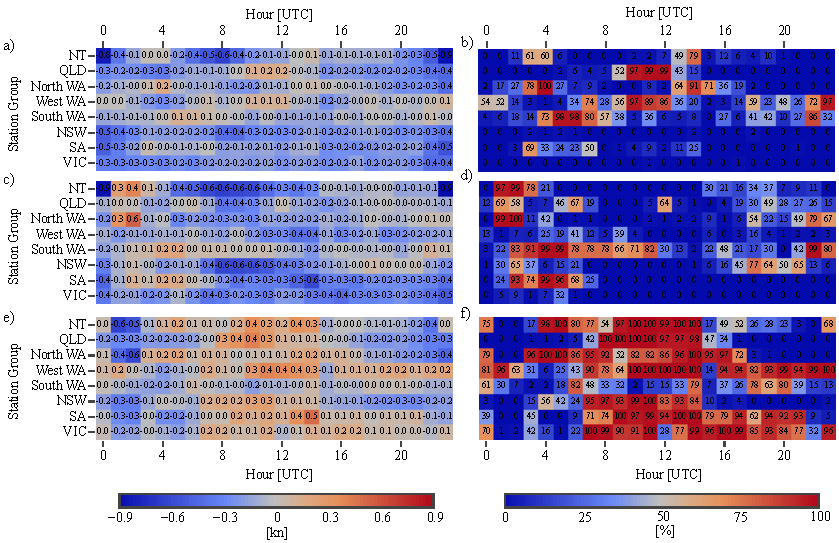
\includegraphics{wpi_coastal.pdf}
\caption{Heatmaps of $\overline{\text{WPI}}$ values and confidence scores for each coastal station group and hour of the day: a) and b), Official versus ACCESS, c) and d) Official versus ECMWF, e) and f) ECMWF versus ACCESS. Positive $\overline{\text{WPI}}$ values mean that the former dataset in each pair is on average closer to observations than the latter dataset. Confidence scores provide the probability the population $\overline{\text{WPI}}$ is greater than zero. Values within the heatmaps are accurate to two significant figures.}
\label{Fig:wpi_coastal}
\end{figure}

Although Official outperforms at least one of ACCESS or ECMWF with high confidence at a few dozen times and station groups, there is only one group and time where it outperforms both. At 05:00 UTC over the South WA station group, $\overline{\text{wpi}}_\text{OA} = 0.2$ kn and $\overline{\text{wpi}}_\text{OE} = 0.1$ kn, both with confidence scores $\geq 95\%$, although the actual $\overline{\text{wpi}}$ values are comparatively small. Note that ECMWF generally outperforms ACCESS from 10:00 - 14:00 UTC, with the South WA station group being the main exception.    

\begin{figure}
\centering
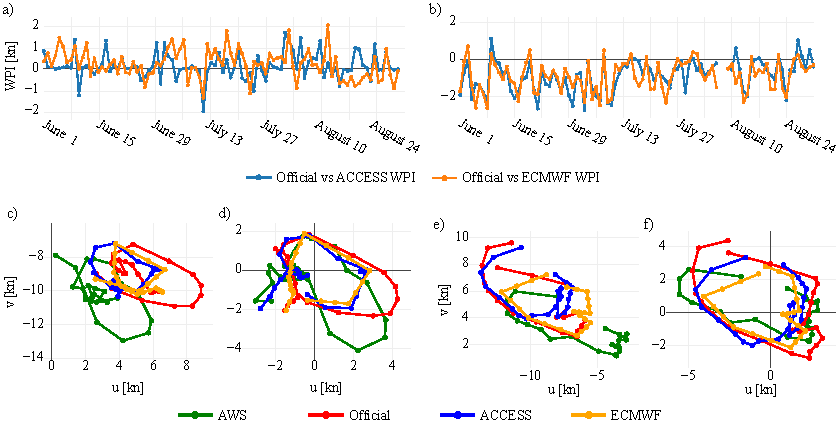
\includegraphics{case_studies.pdf}
\caption{Time series, a) and b), of $\overline{\text{wpi}}_\text{OA}$ and $\overline{\text{wpi}}_\text{OE}$ for, a), the NT station group at 23:00 UTC, and b), the south WA station group at 05:00 UTC. Hodographs, c) to f), showing change in winds, c) and e), and wind perturbations, d) and f), for the NT station group, c) and d), and south WA station group, e) and f).}
\label{Fig:case_studies}
\end{figure}

Using the NT and South WA station groups as case studies, Figures \ref{Fig:case_studies} a) and b) provide time series of $\text{wpi}_\text{OA}$ and $\text{wpi}_\text{OE}$ for, a), the NT station group at 23:00 UTC, and b), the South WA station group at 05:00 UTC. The $\text{wpi}_\text{OA}$ and $\text{wpi}_\text{OE}$ values for the NT station group show significant temporal variability over the three month period, exceeding $-2$ kn on at least 10 days each, and occasionally becoming positive. The $\text{wpi}$ values for the South WA station at 05:00 UTC also show significant temporal variability, with $\text{wpi}_\text{OA}$ and $\text{wpi}_\text{OE}$ each exceeding 1 kn on at least 9 seperate days, despite $\overline{\text{wpi}}_\text{OA}$ and $\overline{\text{wpi}}_\text{OE}$ being small. 

Fig.~\ref{Fig:case_studies} a) shows that there are four days where $\text{wpi}_\text{OA}$ and $\text{wpi}_\text{OE}$ are both less than -2 kn: the 8\textsuperscript{th} of June and the 3\textsuperscript{rd}, 9\textsuperscript{th} and 10\textsuperscript{th} of July. Figures \ref{Fig:case_studies} c) and d) show hodographs of the winds and wind perturbations, respectively, at each hour UTC for the AWS observations, Official forecast, and ACCESS and ECMWF model datasets on the 3\textsuperscript{rd} of July, which provides an interesting example. Figure \ref{Fig:case_studies} e) shows that the Official wind forecast on this day was likely based on edited ACCESS from 00:00 to 06:00 UTC, then edited ECMWF from 07:00 to 13:00 UTC, then unedited ACCESS from 15:00 to 21:00 UTC. The final two hours of the forecast show the Official winds acquiring a stronger east-northeasterly component than either the AWS observations, ACCESS, or ECMWF; this rapid, exaggerated change is even clearer in the perturbation hodograph shown in Fig.~\ref{Fig:case_studies} f). Note that at this time of year the prevailing winds throughout the NT are east-southeasterly, and 22:00 UTC corresponds to $\approx$ 08:30 LST in this region, so the rapid departure of the Official forecast from ACCESS at this time likely represents an edit made by a forecaster to capture boundary layer mixing processes. Figure \ref{Fig:perth_sounding} a) shows the first ten values from wind soundings at Darwin Airport - the nearest station to issue vertical wind soundings - at 12:00 UTC on July 3\textsuperscript{rd} and 00:00 UTC on July 4\textsuperscript{th}. In both instances the winds are indeed east-southeasterly, and so the rapidly changing wind perturbations at 22:00 UTC in the Official forecast likely reflect a boundary layer mixing edit that has been applied either too early, or has strengthened the southeasterly component of the winds too much. The 8\textsuperscript{th} of June and 9\textsuperscript{th} and 10\textsuperscript{th} of July examples are all similar in this respect.              

Considering now the South WA station group, Fig.~\ref{Fig:case_studies} b) shows that $\text{wpi}_\text{OA}$ and $\text{wpi}_\text{OE}$ both exceed 1 kn on the 9\textsuperscript{th} of June and the 3\textsuperscript{rd} of August. Figures \ref{Fig:case_studies} c) and d) show hodographs of the winds and wind perturbations, respectively, at each hour UTC for the AWS observations, Official forecast, and ACCESS and ECMWF model datasets on the 9\textsuperscript{th} of June, which is the more interesting example. The perturbation hodograph shows both ECMWF and ACCESS underpredicting the amplitude of the diurnal wind cycle on this day. In each dataset the 05:00 UTC perturbations are westerly to northwesterly, and given the orientation of the South WA coastline (see Fig.~\ref{Fig:map}) and the fact that 05:00 UTC corresponds to $\approx$ 13:00 local solar time (LST) in this region, the perturbations likely indicate boundary layer mixing processes, rather than the land-sea breeze. Furthermore, the AWS perturbations rapidly become northwesterly between 01:00 and 02:00 UTC, $\approx$ 09:00 - 10:00 LST, which would be about three hours after the sun has risen, consistent with a boundary layer mixing mechanism. 

\begin{figure}
\centering
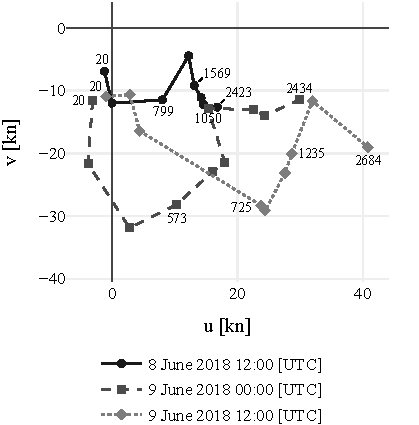
\includegraphics{perth_sounding.pdf}
\caption{Hodographs showing change in winds with height at, a), Darwin Airport, and b), Perth Airport.}
\label{Fig:perth_sounding}
\end{figure}

Figure \ref{Fig:perth_sounding} provides hodographs of wind with height throughout the first two km of the atmosphere between 12:00 UTC on the 8\textsuperscript{th} June and 12:00 UTC on the 9\textsuperscript{th} June; the soundings were taken at Perth Airport, which is the nearest station to the South WA station group to provide wind soundings. The 8\textsuperscript{th} June 12:00 UTC hodograph shows surface northerlies of $\approx 6$ kn, becoming west to northwesterlies of over 20 kn $2.4$ km above the surface. A forecaster basing a model edit of the following days winds on this sounding would therefore gradually strengthen the westerly component of the surface winds in the hours after sunrise. However, the subsequent sounding at 00:00 UTC on the 9\textsuperscript{th} of June shows that the winds acquire a strong northerly component of 30 kn in the first 500 m of the atmosphere, with the final sounding indicating a strong northwesterly wind at 725 m persisting until 12:00 UTC. In Fig.~\ref{Fig:case_studies} d), the Official perturbations from 04:00 to 07:00 UTC show stronger westerly perturbations than either ACCESS or ECMWF, improving the amplitude of Official's diurnal wind cycle. However, the AWS perturbations are more northerly than those of Official, and so the Official forecast winds have been strengthened in a slightly incorrect direction. An explanation for this discrepancy is that the Official forecast for the southwest region of WA has been edited based on the June 8\textsuperscript{th} 12:00 UTC Perth Airport sounding, with the winds above the surface changing direction in the subsequent 12 hours. Note that the 3\textsuperscript{rd} of August example is similar, although in this case the Official forecast slightly improves both the magnitude and direction of the 05:00 UTC wind perturbations.

\begin{figure}
\centering
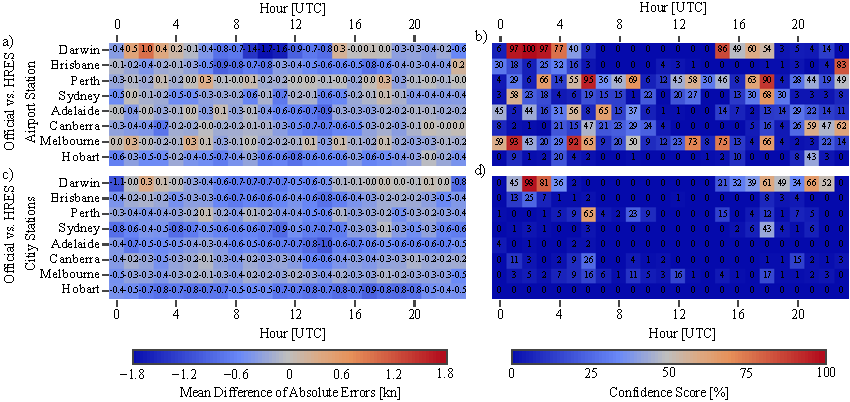
\includegraphics{airport_wpi.pdf}
\caption{The $\overline{\text{wpi}}_\text{OE}$ (Official versus ECMWF comparison) values, a) and c), and confidence scores, b) and d), for the airport stations, a) and b), and airport station groups, c) and d), respectively.}
\label{Fig:airport_wpi}
\end{figure}

Figure \ref{Fig:airport_wpi} presents the $\overline{\text{wpi}}$ values and confidence scores for the Official versus ECMWF comparisons, i.e. $\overline{\text{wpi}}_\text{OE}$ and $P\left(\overline{\text{WPI}}_\text{OE}>0\right)$, for the airport stations, and airport station groups. The results for the airport stations are noisier than the analogous results for the coastal station groups in Figures~\ref{Fig:wpi_coastal} c) and d), although they do share some similarities. Official outperforms ECMWF at 01:00 and 02:00 UTC at both the Darwin airport station and the NT station group, although ECMWF outperforms Official between 08:00 and 14:00 UTC at Darwin and Brisbane airports, and the corresponding NT and QLD station groups, with the exception of the QLD station group at 12:00 UTC where $\overline{\text{wpi}}_\text{OE} = 0$. ECMWF also outperforms Official at Hobart airport at almost all hours of the day, and at Adelaide and Canberra airports from 11:00 to 14:00 UTC. 

For the remaining stations and times, only the Perth airport station at 06:00 UTC and the Melbourne airport station at 01:00 UTC exhibit $\overline{\text{wpi}}_\text{OE}>0$ with $P\left(\overline{\text{WPI}}_\text{OE}>0\right)\geq 95\%$. However, in both cases $\overline{\text{wpi}}_\text{OE}=0.3$, which is small compared to the maximum value of 1.0 which occurs at the Darwin airport station at 02:00 UTC. Furthermore, in both cases there is no clear pattern to the $\overline{\text{wpi}}_\text{OE}$ values over the rest of the day. Given the random appearance of the $\overline{\text{wpi}}_\text{OE}$ values, the \textit{multiplicity problem} \citep[p. 178]{wilks11} requires care be taken before giving meaning to these two examples: i.e., given that we are calculating twenty four confidence scores for eight stations, then assuming WPI were uncorrelated across each station and hour we would expect to find $0.05 \times 24 \times 8 \approx 10$ instances where $P\left(\overline{\text{WPI}}_\text{OE}>0\right)\geq 95\%$, even if $\overline{\text{WPI}}_\text{OE}$ was in fact equal to zero. \textcolor{red}{Comment on performance versus ACCESS.}

For the airport station groups, ECMWF outperforms Official for the majority of station groups and times. The main exception is the Darwin airport station group, where Official outperforms ECMWF at 02:00 UTC, and there is ambiguity as to whether Official or ECMWF performs better at 01:00, 03:00 and 04:00 UTC, and from 15:00 to 22:00 UTC. In the analogous comparisons of Official and ACCESS (not shown), the airport station results are similarly noisy, although the airport station group results are slightly more favourable to Official, with Official outperforming ACCESS from 10:00 to 12:00 UTC at the Brisbane station group, and fewer occasions overall where ACCESS outperforms Official than ECMWF does. 

\begin{figure}
\centering
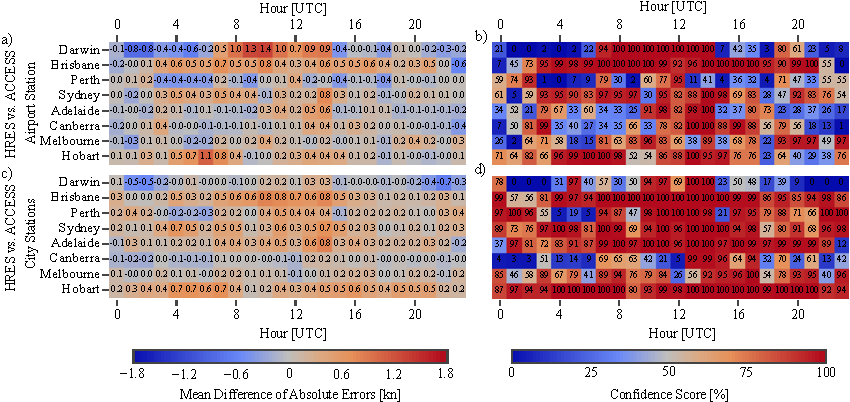
\includegraphics{airport_wpi_EA.pdf}
%\caption{As in Fig.~\ref{Fig:airport_wpi}, but for the $\overline{\text{wpi}}_\text{EA}$ (ECMWF versus ACCESS comparison) values and confidence scores.}
\label{Fig:airport_wpi_EA}
\end{figure}

Figure \ref{Fig:airport_wpi_EA} shows the $\overline{\text{wpi}}$ values and confidence scores for the ECMWF versus ACCESS comparisons, i.e. $\overline{\text{wpi}}_\text{EA}$ and $P\left(\overline{\text{WPI}}_\text{EA}>0\right)$, for the airport stations, and airport station groups. As with the Official versus ECMWF comparison in Fig.~\ref{Fig:airport_wpi}, the results for the airport stations are noisy, but more often than not show that ECMWF outperforms ACCESS. The results for the airport station group show ECMWF usually outperforms ACCESS, the main exceptions being the Darwin and Canberra airport station groups. 

At face value, the fact that ECMWF generally outperforms ACCESS at these scales is surprising, as ACCESS runs at a higher spatiotemporal resolution than ECMWF, and is calibrated for Australian conditions, and so one would expect ACCESS would better resolve small scale processes like the land-sea breeze and boundary layer mixing processes. However, these results are unsurprising if one considers the scales at which predictable atmospheric motion occurs, and the scales being resolved by AWS, ACCESS and ECMWF. The AWS data resolves motion with time scales as low as 10 minutes, and arbitrarily small spatial scales: it therefore includes highly unpredictable eddy turbulence. This explains why the results for the airport stations are noisier than for the airport station groups or coastal station groups. Furthermore, because ACCESS runs at a higher resolution than ECMWF, it includes additional scales of motion, and therefore adds additional variability to the wind fields. Unless this additional variability in ACCESS is perfectly correlated with observations, the average of $\left\lvert \boldsymbol{u}_{\text{AWS}}-\boldsymbol{u}_{\text{A}} \right\rvert$
will therefore increase, unless this additional variability is compensated for by a reduction in bias, i.e.$\left\lvert \overline{\boldsymbol{u}}_{\text{AWS}}-\overline{\boldsymbol{u}}_{\text{A}} \right\rvert$ decreases. These ideas are discussed in greater detail in section \ref{Sec:Discussion}. Note finally that the results for the Official versus ECMWF comparison in Fig.~\ref{Fig:airport_wpi} largely mirror those of the ECMWF versus ACCESS comparison in Fig.~\ref{Fig:airport_wpi_EA}, e.g. for the Darwin airport station and station group, Official outperforms ECMWF at the same times that ACCESS does, suggesting that either the Official forecast at these spatial scales is largely based on ACCESS, or that ECMWF is highly biased at these scales and times.

\subsection{Seasonal Comparison}
\label{Sec:Seasonal}
Figure \ref{Fig:cwpi_coastal} provides the climatological wind perturbation index values, $\text{cwpi}$, and confidence scores, $P\left(\text{CWPI}>0\right)$, for the coastal station groups for $\text{cwpi}_\text{OA}$, $\text{cwpi}_\text{OE}$ and $\text{cwpi}_\text{EA}$, which represent the the Official versus ACCESS, Official versus ECMWF, and ECMWF versus ACCESS comparisons, respectively. At the NT station group Official outperforms both ACCESS and ECMWF at 03:00 UTC with $\text{cwpi}_\text{OA} = \text{cwpi}_\text{OE} = 0.4$, $P\left(\text{cwpi}_\text{OA}>0\right) = 94\%$ and $P\left(\text{cwpi}_\text{OE}>0\right) = 93\%$. However, both ACCESS and ECMWF outperform Official at 23:00 and 00:00 UTC, consistent with the $\overline{\text{wpi}}$ results in Fig.~\ref{Fig:wpi_coastal}. The NT station group results are discussed in more detail in section \ref{Sec:Discussion}.

At the North WA station group at 01:00, 03:00 and 04:00, Official outperforms ACCESS with confidence scores of 77, 78 and 90\%, respectively; Official also outperforms ECMWF at 01:00 and 02:00 UTC with confidence scores above 99\%. Figure \ref{Fig:clim_hodo} a) shows that ECMWF's poor performance at 01:00 and 02:00 UTC is simply due to its linear interpolation at these times, whereas Official's outperformance of ACCESS at 01:00, 03:00 and 04:00 is due to ACCESS's climatological diurnal cycle being slightly out of phase with that of the AWS observations, and the Official forecast appearing to correct for this somewhat. Both Official and ECMWF slightly exaggerate the magnitude of the climatological sea-breeze with ACCESS doing a good job in this regard.    

At the South WA station group from 01:00 to 05:00 UTC, $\text{cwpi}_\text{OE}$ is positive with confidence scores of at least $88\%$, although $\text{cwpi}_\text{OA}$ is negative or zero at these times. Figure \ref{Fig:clim_hodo} b) shows that ECMWF underestimates the westerly perturbations at these times, with these perturbations likely associated with boundary layer mixing processes, as discussed in section \ref{Sec:Daily}. Each of Official, ACCESS and ECMWF underestimate the amplitude of the diurnal cycle between 02:00 and 10:00 UTC, including both the westerly perturbations and the southerly sea-breeze perturbations. 

At the NSW station group from 17:00 to 19:00 UTC, $\text{cwpi}_\text{OA}$ and $\text{cwpi}_\text{OE}$ are at least $0.4$ and $0.1$ kn, respectively, with confidence scores of at least 95\% and 75\%, respectively. Figure \ref{Fig:clim_hodo} c) shows that these times correspond to a strange ``dimple" in perturbation hodograph that is present in all four datasets. The Official hodograph closely resembles that of ACCESS, except for this dimple, which has been exaggerated relative to ACCESS. \textcolor{red}{Don't know what is going on here.} Figure \ref{Fig:clim_hodo} c) also shows that although ECMWF exaggerates the amplitude of the easterly sea-breeze perturbations, it captures the narrower shape of the AWS hodograph better than Official or ACCESS. 

At the SA station group from 01:00 to 05:00 UTC and 09:00 to 11:00 UTC both $\text{cwpi}_\text{OA}$ and $\text{cwpi}_\text{OE}$ are positive, with maximum values of $0.4$ and $0.1$ kn, although confidence scores do not exceed 88\% and 65\% respectively. Figure \ref{Fig:clim_hodo} shows that the Official forecast captures the amplitude of the perturbations from 01:00 to 05:00 UTC almost perfectly, matching the amplitude of the AWS perturbations better than both ACCESS and ECMWF. However, the Official diurnal cycle is slightly out of phase with the AWS cycle during this period, explaining why Official only slightly outperforms ACCESS in the results of Figures \ref{Fig:cwpi_coastal} a) and b).      

\begin{figure}
\centering
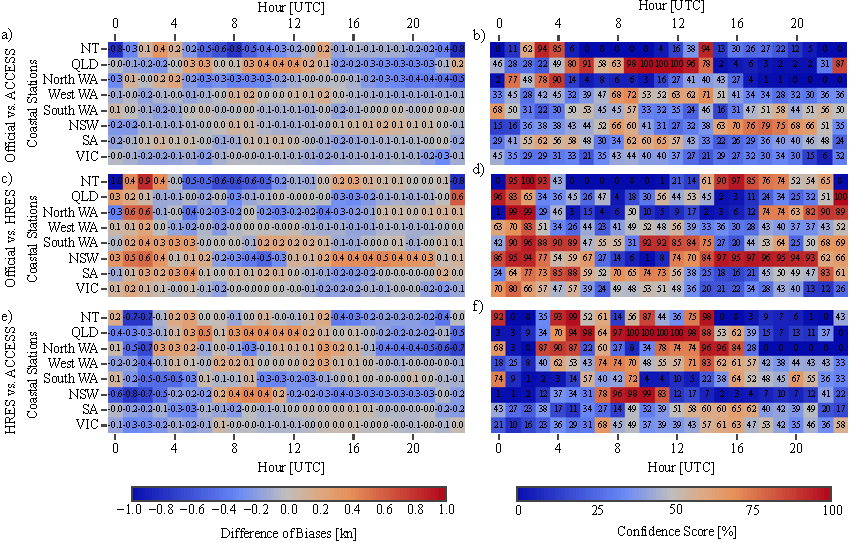
\includegraphics{cwpi_coastal.pdf}
%\caption{As in Fig.~\ref{Fig:wpi_coastal}, but for the values and confidence scores.}
\label{Fig:cwpi_coastal}
\end{figure}

\begin{figure}
\centering
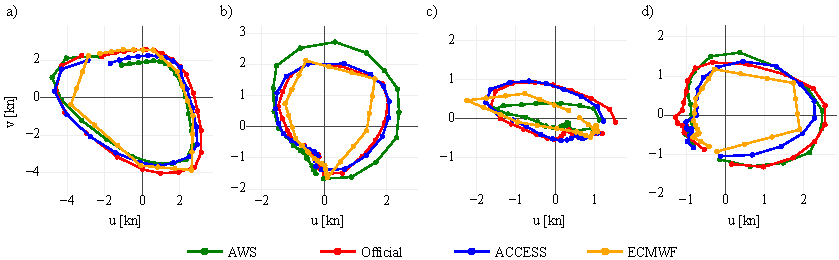
\includegraphics{clim_hodo.pdf}
\caption{Climatological hodographs.}
\label{Fig:clim_hodo}
\end{figure}

While the $\text{cwpi}$ values and confidence scores of Fig.~\ref{Fig:cwpi_coastal} provide detailed information on which dataset's climatological diurnal cycle best matches those of the AWS observations, $\text{cwpi}$ on it's own reveals little about the structure of the diurnal cycle, and provides little insight into forecast accuracy could be improved. Note that the hodographs in Fig.~\ref{Fig:clim_hodo} are roughly elliptical in shape, suggesting that descriptive quantities can be estimated by fitting equations (\ref{Eq:u}) and (\ref{Eq:v}) to the zonal and meridional climatological perturbations, then calculating these quantities from the fit, as described in section \ref{Sec:Methods}. 

\begin{figure}
\centering
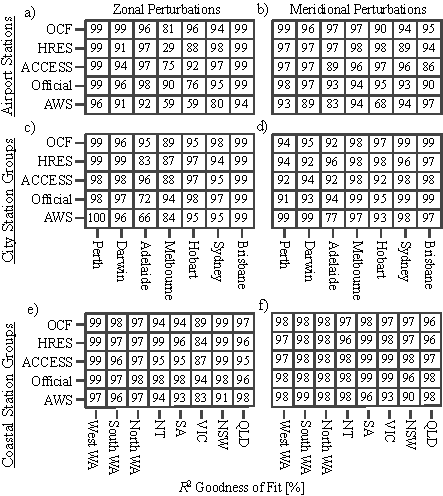
\includegraphics{r_squared.pdf}
\caption{\textcolor{red}{Could also provide an analogous figure showing the use of the function $\alpha$ provides a significant improvement over the basic ellipse fit - or instead just quote some numbers? Or maybe these figures are entirely unnecessary?}}
\label{Fig:r_squared}
\end{figure}

Figure \ref{Fig:r_squared} provides the $R^2$ values for the fits of the zonal and meridional perturbations to equations (\ref{Eq:u}) and (\ref{Eq:v}), respectively. The fit performs best at the coastal station group spatial scale, with $R^2$ generally above $95\%$. It also performs well at the airport station and airport station group scales, with a few exceptions, including the ACCESS and Official meridional perturbations at the Canberra airport station group, and the ECMWF zonal perturbations at Melbourne airport. 

\begin{figure}
\centering
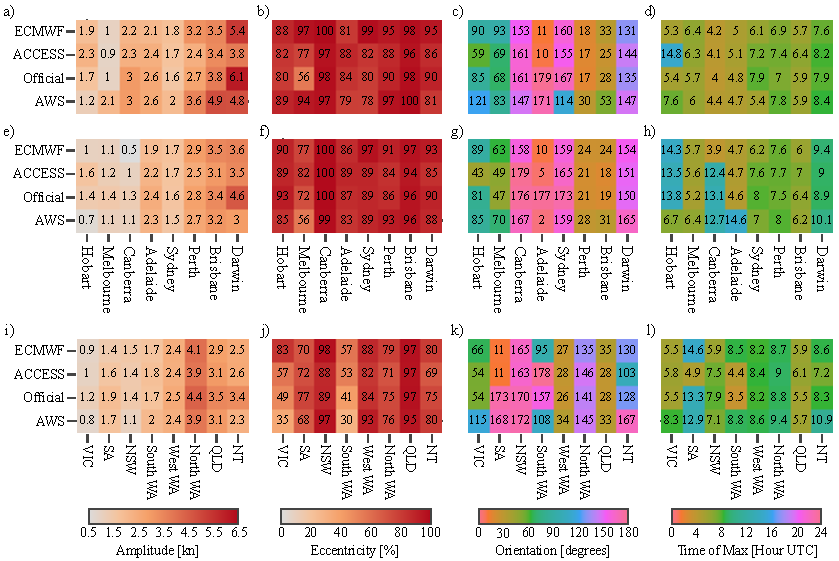
\includegraphics{ellipse_fits.pdf}
\caption{Ellipse fits. \textcolor{red}{If we were to include any analysis for alternative time periods (e.g. summer 2017/18 for contrast; or could do 18/19 if I were to go back to BoM to get the data) a copy of this figure could be a good choice. Could explain changes in diurnal cycle properties, e.g. amplitude, with seasonal changes to background winds, heating, etc.}}
\label{Fig:ellipse_fits}
\end{figure}

The ellipse fits are used to derive four descriptive quantities: amplitude (half the length of the semi-major axis), eccentricity, orientation (the angle the semi-major axis makes with lines of latitude) and the time of the peak in the diurnal cycle (the time at which the perturbations align with the semi-major axis, ignoring translational coefficients). Figure \ref{Fig:ellipse_fits} provides these four quantities for each dataset and location across the three spatial scales. A variety of structural differences are apparent at a number of locations and scales. For instance, Fig.~\ref{Fig:ellipse_fits} a) shows that at Brisbane airport, the amplitude of the AWS diurnal cycle is at least $1$ kn greater than Official, ACCESS and ECMWF, and Fig.~\ref{Fig:ellipse_fits} c) shows that the orientation of the AWS diurnal cycle hodograph is at least 20 degrees (anti-clockwise) from the other datasets. Figures \ref{Fig:ellipse_hodo} a) and b) show hodographs of the Brisbane airport perturbation climatology and ellipse fit, respectively. Although the ellipse fit suppresses some of the asymmetric details, it captures the amplitudes and orientations of the real climatological diurnal cycles well. In this case the results show that the average AWS sea-breeze approaches from the northeast, whereas the forecast and model sea-breezes approach more from the east-northeast. To check whether this just represents a direction bias of the Brisbane Airport station, Fig.~\ref{Fig:ellipse_fits} shows the climatological perturbations at the nearby Spitfire Channel station (see Fig.~\ref{Fig:maps} for the location of this station, and other stations referred to in this section).   

\begin{figure}
\centering
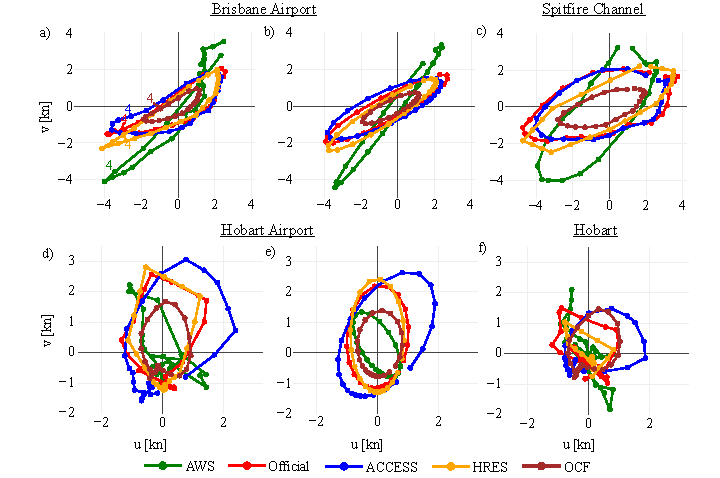
\includegraphics{ellipse_hodo.pdf}
\caption{Ellipse fits. Could instead just provide one example.}
\label{Fig:ellipse_hodo}
\end{figure}

\begin{figure}
\centering
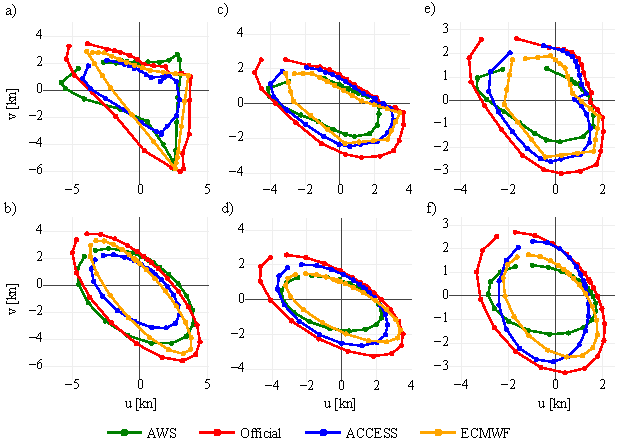
\includegraphics{nt_ellipse_hodo.pdf}
\caption{Ellipse fits. Could instead not include the ellipses.}
\label{Fig:ellipse_hodo}
\end{figure}


\begin{comment}
Four examples? Brisbane airport definitely. Can show Darwin Airport hodographs in discussion section. Hobart airport or Hobart airport group. Why not just two examples? Spitfire channel very similar!}
\end{comment}

\section{Discussion}
\label{Sec:Discussion}
The methods developed in this study can be readily extended to analyse \emph{just} the sea-breezes satisfying the operational definition above. For instance, to study the sea-breezes at a station near a coastline with inward pointing normal vector $\widehat{\boldsymbol{n}}$, the wind perturbation datasets could be restricted to just those days where the corresponding raw wind vector $\boldsymbol{u}$ satisfies $\widehat{\boldsymbol{n}} \cdot \boldsymbol{u} > 0$ for at least one of the hours of that day.

How much time should forecasters spend on sea-breeze edits (if any)? What is the value of an improved diurnal cycle climatology? Improving the accuracy of forecast climatologies will have little value to the typical forecast user. Are there applications where a higher performing climatological forecast yields better outcomes, even if errors increase or even get worse? 

Increasing the resolution of a forecast may reduce bias, but increase error.

Error, not bias, that generally matters for the forecast user. Standard methods for ``improving" forecasts (adding parametrisations, increasing resolution) reduce bias, but actually increase errors! 

Although they have similar definitions, $\overline{\text{WPI}}$ and CWPI measure different things. They do not converge as the length of the time period grows - they don't even necessarily approach the same sign. As a simple example, suppose that for each day, the observed and Official wind perturbations are given by $\boldsymbol{p}_{\text{AWS}} = \left(5\cos\omega t , 5\sin\omega t\right)$ and $\boldsymbol{p}_\text{O} = \left(6\cos\omega t , 6\sin\omega t\right)$, respectively. Furthermore, suppose that the ACCESS perturbations alternate between $\boldsymbol{p}_{\text{A}} = \left(7\cos\omega t , 7\sin\omega t\right)$ and $\boldsymbol{p}_{\text{A}} = \left(3\cos\omega t , 3\sin\omega t\right)$ from one day to the next. Then for any contiguous period of $n$ days, $\overline{\text{WPI}} = 2 - 1 = 1$, but $\text{CWPI} \approx -1$, with the approximation becoming exact for even $n$. Moreover $\overline{\text{WPI}}=1$ with a confidence of 1, and using the bootstrapping procesure described above, the confidence that $\text{CWPI} = -1$ approaches 1 as $n\to \infty$. This example shows that while the WPI and CWPI are sensitive both to random error and consistent biases between the different datasets, the CWPI becomes increasingly less sensitive to random error as the length of the time period being considered grows. Thus while the WPI arguably provides a more meaningful operational metric, as it measures the accuracy of actual forecast data, it may favour a more biased dataset over a less biased one, just because the internal variability of that dataset is lower. One consequence of this is that model data at a lower spatiotemporal resolution may outperform in $\overline{\text{WPI}}$ model data of a higher resolution, purely because the internal variability is lower. In this way, the CWPI may actually provide more information about the performance of different forecasts.

Note that the Bureau has not yet moved to ensemble forecasting - and probabilistic verification methods are therefore not appropriate. 

\begin{figure}
\centering
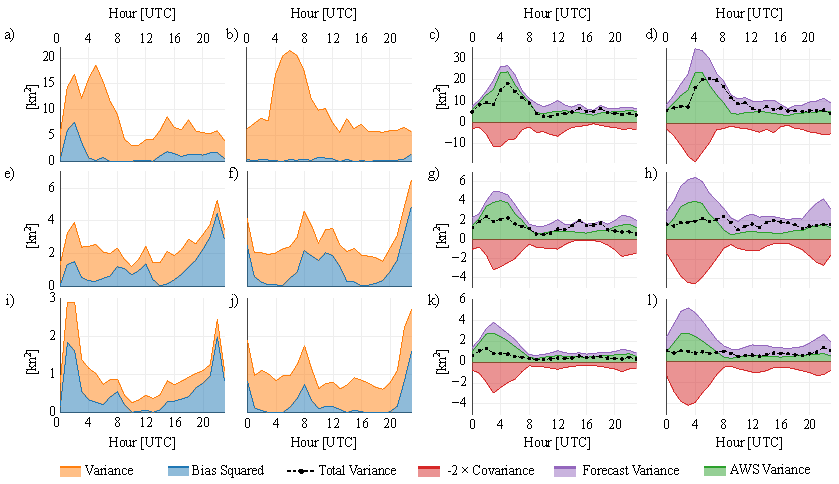
\includegraphics{error_decomp.pdf}
\caption{Actual perturbation standard deviation values. Note that official performs the worst at this scale!}
\label{Fig:error_decomp}
\end{figure}

\begin{figure}
\centering
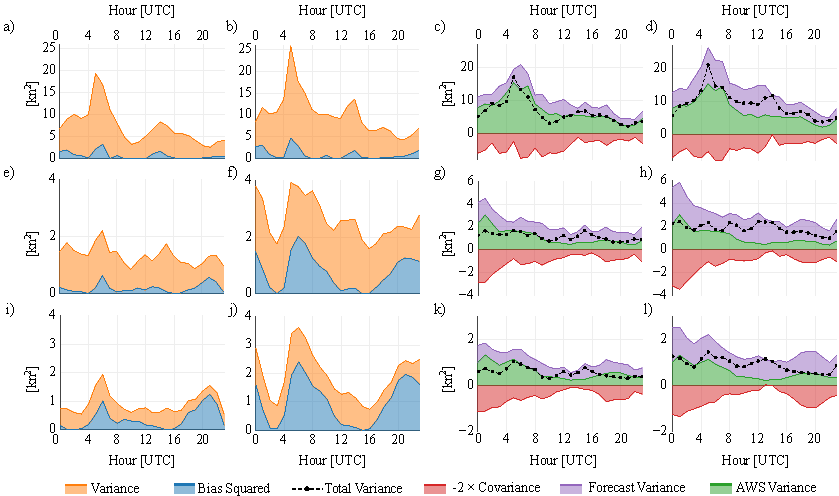
\includegraphics{error_decomp_v.pdf}
\caption{Actual perturbation standard deviation values. Note that official performs the worst at this scale!}
\label{Fig:error_decomp_v}
\end{figure}

\section{Conclusion}
\label{conclusion}
In this report, a methodology for comparing the performance of Bureau forecasts of diurnal wind processes to unedited model guidance products has been developed and applied to a case study of the Darwin airport. The key results may be summarised as follows.
\begin{enumerate}
\item
During the dry season months of June, July and August 2017, the ECMWF sea-breeze is generally more accurate than that of the official forecast. However, during the wet season months of December, January and February 2017/18 this result is reversed, and the official forecast sea-breeze generally outperforms that of ECMWF. 
\item
In both seasons, boundary layer mixing processes are generally represented better in official forecasts than in ECMWF.
\item
In the dry season, the climatological wind perturbations of the official forecast generally outperform those of ECMWF between 13:00 and 16:00 UTC. This is due to ECMWF not capturing the magnitude of the south-easterly mean perturbations. 
\item
During the wet season, the climatological wind perturbations of the official forecast generally outperform those of ECMWF at 11:00 UTC. This is due to ECMWF underestimating the magnitude of the mean land-breeze perturbation.
\end{enumerate}

There a number of ways that this work could be extended. The most pressing would probably be to investigate whether the results presented here change when a more operational definition of the sea breeze is used in place of the entirely perturbation based definition used here: this could be done using the method described in section \ref{methods}.

\bibliography{./references.bib}

\end{document}
